\documentclass{beamer}
\usepackage{verbatim}
\usepackage{booktabs}
\usepackage{multirow}
\usepackage{graphicx}
\usepackage{subcaption}
\graphicspath{{./figures}}

\usetheme{Madrid}
\title{Awesome Modeling}
\institute{University of Padua}
\date{AY 2023/2024}

\makeatletter
% Remove navigation symbols
\setbeamertemplate{navigation symbols}{}
\makeatother

\author[Basaglia, Popović, Stocco]
{A.~Basaglia\inst{1} \and M.~Popović\inst{1} \and A.~Stocco\inst{1}}

\institute[UniPD]
{
  \inst{1}
  University of Padua
}

\begin{document}

\frame{\titlepage}

\begin{frame}
\frametitle{Table of Contents}
\tableofcontents
\end{frame}

\section{Introduction}
\begin{frame}{Introduction}
\textit{The project’s objective is to build a platform for obtaining articles
from online newspapers, storing them, making them searchable, and
extracting representations of themes discussed in a set of articles
returned as results for a given query.}
\end{frame}

\section{Architecture}
\begin{frame}{Architecture}
\begin{figure}[ht]
    \centering
    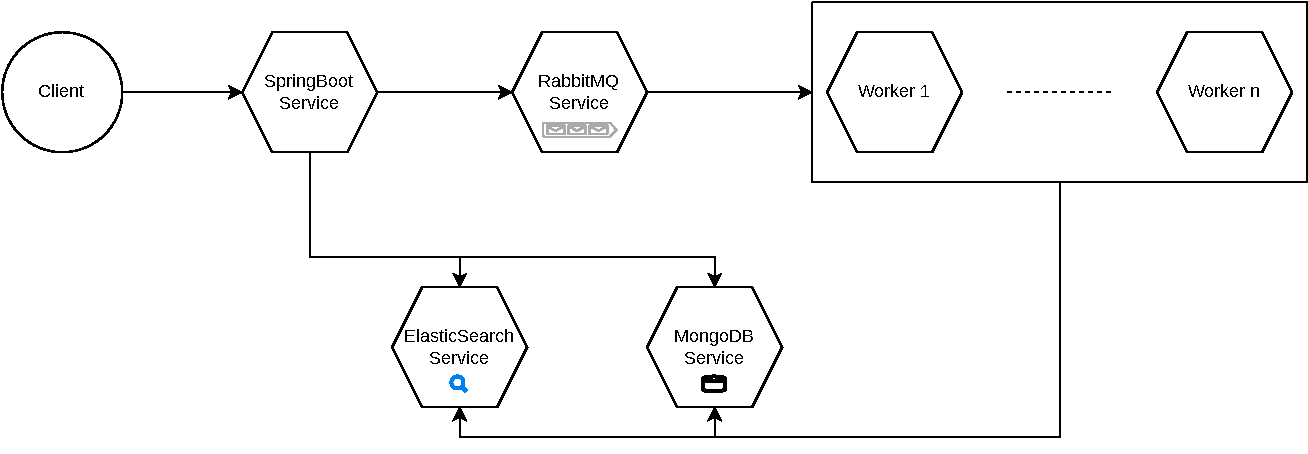
\includegraphics[width=1\linewidth] {microservices.drawio.pdf}
    \caption{Microservices}
    \label{fig:microservices}
\end{figure}
\end{frame}

\section{Sequence Diagram}
\begin{frame}{Sequence Diagram}
\begin{figure}[ht]
    \centering
    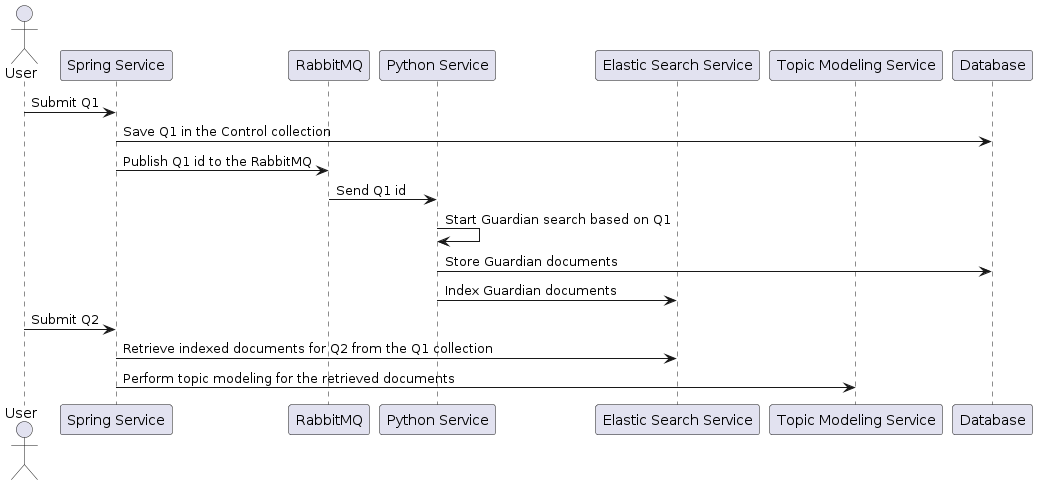
\includegraphics[width=0.7\linewidth]{figures/sequenceDiagram.png}
    \caption{Sequence diagram}
    \label{fig:seqDiagram}
\end{figure}
\end{frame}

\section{Design choices}
\begin{frame}{Design choices}
\begin{itemize}
    \item Downloading and indexing are \textbf{Asynchronous}
    \item \textbf{Scalability} improved
\end{itemize}
\end{frame}

\section{Conclusions}
\begin{frame}{Conclusions}
\centering
Let's see a demo!
\end{frame}

\end{document}
